% This file was created by tikzplotlib v0.8.1.
\begin{figure} [H]
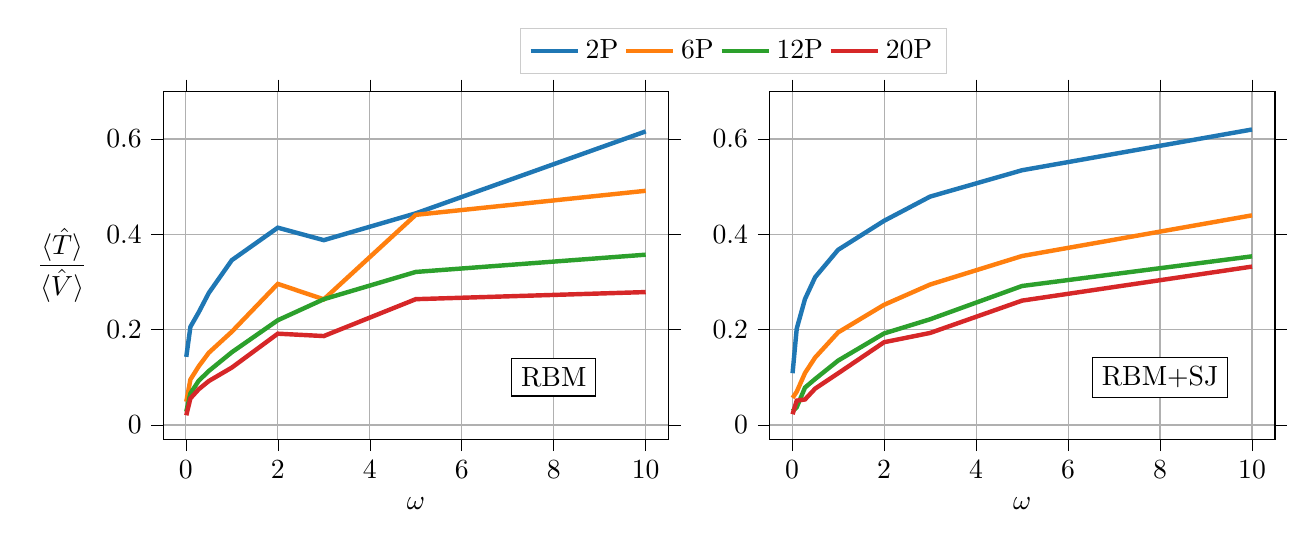
\begin{tikzpicture}

\definecolor{color0}{rgb}{0.12156862745098,0.466666666666667,0.705882352941177}
\definecolor{color1}{rgb}{1,0.498039215686275,0.0549019607843137}
\definecolor{color2}{rgb}{0.172549019607843,0.627450980392157,0.172549019607843}
\definecolor{color3}{rgb}{0.83921568627451,0.152941176470588,0.156862745098039}

\begin{axis}[
legend cell align={left},
legend style={at={(1.55,1.05)}, anchor=south east, draw=white!80.0!black},
legend columns = 4,
tick align=outside,
tick pos=both,
x grid style={white!69.01960784313725!black},
xlabel={\(\displaystyle \omega\)},
width=8cm,
height=6cm,
xmajorgrids,
xmin=-0.4895, xmax=10.4995,
xtick style={color=black},
y grid style={white!69.01960784313725!black},
ylabel style={rotate=-90.0},
ylabel={\(\displaystyle \frac{\langle\hat{T}\rangle}{\langle\hat{V}\rangle}\)},
ymajorgrids,
ymin=-0.03, ymax=0.7,
ytick style={color=black}
]
\addplot [ultra thick, color0]
table {%
0.01 0.14292980671414
0.1 0.206000508517671
0.28 0.236346842166032
0.5 0.277065579844387
1 0.345784185233727
2 0.41399969664796
3 0.387796539576211
5 0.444067718952601
10 0.616027732463295
};
\addlegendentry{2P}
\addplot [ultra thick, color1]
table {%
0.01 0.0489614243323442
0.1 0.0953652097389264
0.28 0.123020257826888
0.5 0.151552210724365
1 0.195728715728716
2 0.296060131091479
3 0.263623577547628
5 0.440925380415408
10 0.491388484677367
};
\addlegendentry{6P}
\addplot [ultra thick, color2]
table {%
0.01 0.0279279279279279
0.1 0.0663141106354403
0.28 0.0927190456602221
0.5 0.113307273027584
1 0.152620094780267
2 0.21978952717725
3 0.263891885843983
5 0.321107495449782
10 0.357318784099766
};
\addlegendentry{12P}
\addplot [ultra thick, color3]
table {%
0.01 0.0202855736090596
0.1 0.0558188176084186
0.28 0.0748673013733255
0.5 0.092181964299863
1 0.120447174205168
2 0.191577362501107
3 0.186589637000426
5 0.263982205508037
10 0.278872126802915
};
\addlegendentry{20P}

\node[draw,fill=white] at (axis cs: 8,.1) {RBM};
\end{axis}

\begin{axis}[
xshift=7.7cm,
legend cell align={left},
legend style={at={(0.97,0.03)}, anchor=south east, draw=white!80.0!black},
tick align=outside,
tick pos=both,
x grid style={white!69.01960784313725!black},
xlabel={\(\displaystyle \omega\)},
xmajorgrids,
width=8cm,
height=6cm,
xmin=-0.4895, xmax=10.4995,
xtick style={color=black},
y grid style={white!69.01960784313725!black},
%ylabel style={rotate=-90.0},
%ylabel={\(\displaystyle \frac{\langle\hat{T}\rangle}{\langle\hat{V}\rangle}\)},
ymajorgrids,
ymin=-0.03, ymax=0.7,
ytick style={color=black}
]
\addplot [ultra thick, color0]
table {%
	0.01 0.108705258506407
	0.1 0.202009646302251
	0.28 0.264296187683284
	0.5 0.310018755861207
	1 0.367553865652725
	2 0.428427393293865
	3 0.479188481675393
	5 0.534512711346008
	10 0.620005473453749
};
%\addlegendentry{2P}
\addplot [ultra thick, color1]
table {%
	0.01 0.0567119155354449
	0.1 0.0697142186491403
	0.28 0.109019214224262
	0.5 0.141514485132422
	1 0.194234043802478
	2 0.252176075603084
	3 0.294666494223597
	5 0.354539716887567
	10 0.439893538370546
};
%\addlegendentry{6P}
\addplot [ultra thick, color2]
table {%
	0.01 0.0288659793814433
	0.1 0.0372200263504611
	0.28 0.0784915858002702
	0.5 0.096412072256494
	1 0.135095692138839
	2 0.192092791484218
	3 0.221784714644907
	5 0.291641379310345
	10 0.353855680855225
};
%\addlegendentry{12P}
\addplot [ultra thick, color3]
table {%
	0.01 0.0224807471735212
	0.1 0.0510365183964855
	0.28 0.0535270823545204
	0.5 0.0761996706229769
	1 0.108428284656055
	2 0.17366909653192
	3 0.19307880632568
	5 0.260942252768941
	10 0.332349732889548
};
%\addlegendentry{20P}
\node[draw, fill=white] at (axis cs: 8,.1) {RBM+SJ};
\end{axis}

\end{tikzpicture}

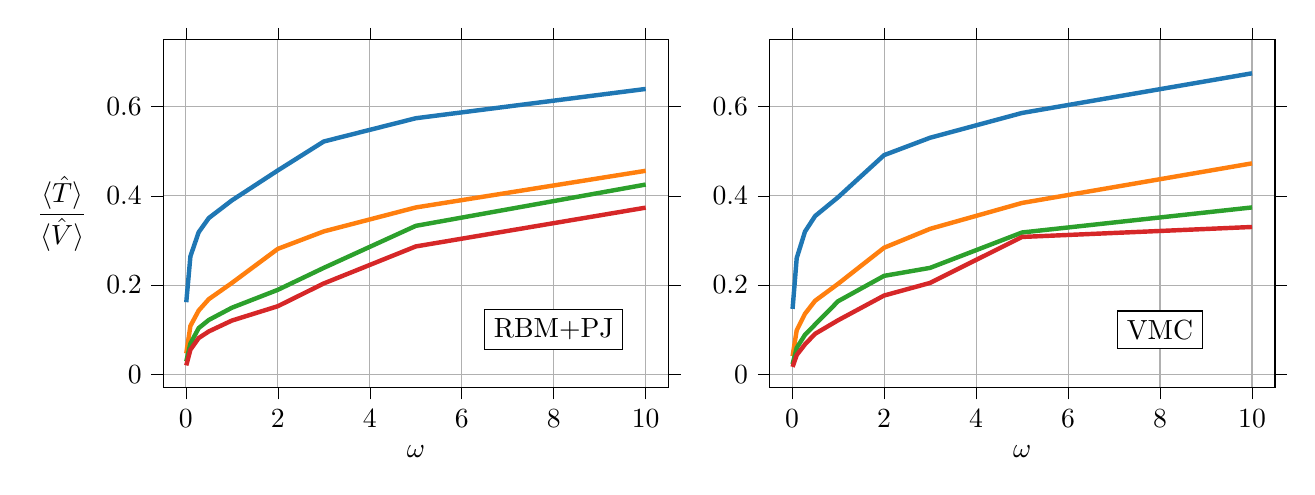
\begin{tikzpicture}

\definecolor{color0}{rgb}{0.12156862745098,0.466666666666667,0.705882352941177}
\definecolor{color1}{rgb}{1,0.498039215686275,0.0549019607843137}
\definecolor{color2}{rgb}{0.172549019607843,0.627450980392157,0.172549019607843}
\definecolor{color3}{rgb}{0.83921568627451,0.152941176470588,0.156862745098039}

\begin{axis}[
legend cell align={left},
legend style={at={(0.97,1.03)}, anchor=south east, draw=white!80.0!black},
tick align=outside,
tick pos=both,
x grid style={white!69.01960784313725!black},
xlabel={\(\displaystyle \omega\)},
width=8cm,
height=6cm,
xmajorgrids,
xmin=-0.4895, xmax=10.4995,
xtick style={color=black},
y grid style={white!69.01960784313725!black},
ylabel style={rotate=-90.0},
ylabel={\(\displaystyle \frac{\langle\hat{T}\rangle}{\langle\hat{V}\rangle}\)},
ymajorgrids,
ymin=-0.03, ymax=0.75,
ytick style={color=black}
]
\addplot [ultra thick, color0]
table {%
	0.01 0.161598746081505
	0.1 0.264466364626943
	0.28 0.318533815178111
	0.5 0.350256285086649
	1 0.389730328777244
	2 0.456965583072599
	3 0.52190696776684
	5 0.574018126888218
	10 0.639722703639515
};
%\addlegendentry{2P}
\addplot [ultra thick, color1]
table {%
	0.01 0.0468986384266263
	0.1 0.108489101409675
	0.28 0.142927927927928
	0.5 0.168400011874487
	1 0.204595643091614
	2 0.281150742944763
	3 0.320306803143652
	5 0.373984932084395
	10 0.456212770963223
};
%\addlegendentry{6P}
\addplot [ultra thick, color2]
table {%
	0.01 0.0287417763157895
	0.1 0.0689267491135519
	0.28 0.103510351035104
	0.5 0.121754035137837
	1 0.149081447331657
	2 0.189290836653386
	3 0.238556500646571
	5 0.332749562171629
	10 0.425379527774922
};
%\addlegendentry{12P}
\addplot [ultra thick, color3]
table {%
	0.01 0.0198390540318607
	0.1 0.0550696242390316
	0.28 0.0812272164373049
	0.5 0.0960548685344326
	1 0.120346512979882
	2 0.152555093728466
	3 0.20363356015151
	5 0.286590458917023
	10 0.373618884667807
};
%\addlegendentry{20P}
\node[draw,fill=white] at (axis cs: 8,.1) {RBM+PJ};
\end{axis}

\begin{axis}[
xshift=7.7cm,
legend cell align={left},
legend style={at={(0.97,0.03)}, anchor=south east, draw=white!80.0!black},
tick align=outside,
tick pos=both,
x grid style={white!69.01960784313725!black},
xlabel={\(\displaystyle \omega\)},
xmajorgrids,
width=8cm,
height=6cm,
xmin=-0.4895, xmax=10.4995,
xtick style={color=black},
y grid style={white!69.01960784313725!black},
%ylabel style={rotate=-90.0},
%ylabel={\(\displaystyle \frac{\langle\hat{T}\rangle}{\langle\hat{V}\rangle}\)},
ymajorgrids,
ymin=-0.03, ymax=0.75,
ytick style={color=black}
]
\addplot [ultra thick, color0]
table {%
	0.01 0.146594427244582
	0.1 0.260418749464423
	0.28 0.319901846829394
	0.5 0.354717597127
	1 0.396972519795063
	2 0.491318502441671
	3 0.53027950310559
	5 0.585870116692034
	10 0.67481056582395
};
%\addlegendentry{2P}
\addplot [ultra thick, color1]
table {%
	0.01 0.0407722122838402
	0.1 0.0985104942450914
	0.28 0.135666711367395
	0.5 0.164801025691602
	1 0.202835527491511
	2 0.28369079862382
	3 0.326016767506851
	5 0.384115256741781
	10 0.472868887927304
};
%\addlegendentry{6P}
\addplot [ultra thick, color2]
table {%
	0.01 0.0225470925470925
	0.1 0.0591952540624194
	0.28 0.0885030700825746
	0.5 0.111576919808515
	1 0.163770657314416
	2 0.220633968028807
	3 0.238556500646571
	5 0.317885405699147
	10 0.37406475534662
};
%\addlegendentry{12P}
\addplot [ultra thick, color3]
table {%
	0.01 0.0164511376657391
	0.1 0.0430938843433643
	0.28 0.067074638154502
	0.5 0.0907330085826954
	1 0.121087634122869
	2 0.176534004132603
	3 0.20481414099371
	5 0.307872099467483
	10 0.330233868695407
};
%\addlegendentry{20P}
\node[draw, fill=white] at (axis cs: 8,.1) {VMC};
\end{axis}

\end{tikzpicture}
\caption{The kinetic-potential energy ratio $\langle\hat{T}\rangle/\langle\hat{V}\rangle$ plotted as a function of the oscillator frequency for two-dimensional circular quantum dots. The frequencies $\omega=0.01,$ 0.1, 0.28, 0.5, 1.0, 2.0, 3.0, 5.0, 10.0 were run. The methods used were detailed in the introductory words of this chapter.}
\label{fig:energydistribution}
\end{figure}